\chapter{Creating Good Graphics}
\label{ch:graphics}


It is essential to use high-quality, efficiently sized figures (aka
``graphics'').
You may be asked to re-make any that egregiously violate some some
basic standards.
These standards are in place to avoid sub-optimal figures, bloated
files sizes, and delayed publishing schedules.  E.g., the arXive puts a limit of 10\,MB on documents.

Often the best thing to do is to \textbf{not} process or attempt to
optimize a graphic but provide the editors access to the most ``raw''
graphic which your software can produce.
If at all uncertain, please contact the technical editors.
The rest of this section provides guidance on how to create optimal
figures.

%%%%%%%%%%%%%%%%%%%%%%%%%%%%%%%%%%%%%%%%%%%%%%%%%%%%%%%%%%%%%%%%%%%%
\section{Graphic Types}
\label{sec:graphic-types}

There two basic graphic content types; these are important to understand:

\begin{description}
\item[raster] a two dimensional array of pixels
\item[vector] a two dimensional drawing description language
\end{description}

The documents compile with \texttt{pdflatex} and so may use graphics
in PDF, JPEG or PNG file formats.
These formats have specific best uses:

\begin{description}
\item[JPEG] use for photographs
\item[PDF] use of any line drawings, plots, illustrations
\item[PNG] use due to some inability to produce proper JPEG or PDF (contact editors)
\end{description}

It is possible (though unwise) to store inherently raster information
in PDF or to rasterize inherently vector information into JPEG or PNG.
\textbf{This is the main cause for bloated, low-quality graphics.}
Here are some guidelines addressing this common problem:

\begin{itemize}
\item Only save photographic images to JPEG, avoid re-saves.
\item Save line drawings, plots or illustrations directly to vector PDF.
\item Follow special guidance on annotation (see Section~\ref{sec:graphic-annotate}).
\item Never convert any raster data (JPEG/PNG) to PDF.
\item Never raster what is really vector data in to a JPEG/PNG.
\item Never use MicroSoft PowerPoint for any figure as it tends to lead to poor quality and bloated files.
\item Do save using native application formats to allow later
  modification
\item Leave any potential format conversions to the technical editors.
\item Consider providing plots as easy-to-reproduce ROOT, Python or
  other scripts.
  (see Section~\ref{sec:graphic-plots})
\end{itemize}

\noindent If authors find these guidelines can not be followed for any
given graphic, please contact the technical editors.   

%%%%%%%%%%%%%%%%%%%%%%%%%%%%%%%%%%%%%%%%%%%%%%%%%%%%%%%%%%%%%%%%%%%%
\section{Plots}
\label{sec:graphic-plots}

Where possible, it is recommended that any plots be submitted in a
form that allows easy reproduction from data in the course of building
the document.
This allows the technical editors to attempt to apply consistent
in-plot fonts, colors, wording.
\fixme{More info to be added.}

%%%%%%%%%%%%%%%%%%%%%%%%%%%%%%%%%%%%%%%%%%%%%%%%%%%%%%%%%%%%%%%%%%%%
\section{Annotated Figures}
\label{sec:graphic-annotate}

It is a common activity to take a figure and annotate it with arrows, labels, etc.
For example, as shown in Figure \ref{fig:annotation-original}, annotations were made on a decaying kaon in the ICARUS T600 detector
considered in a PDK analysis. Then shown again with similar markups after using the \LaTeX{} TikZ package in Figure \ref{fig:annotation-tikz}.

\begin{dunefigure}[Annotations: original graphic]{fig:annotation-original}{An image annotated by, for example Powerpoint, often leading to file size bloat.}
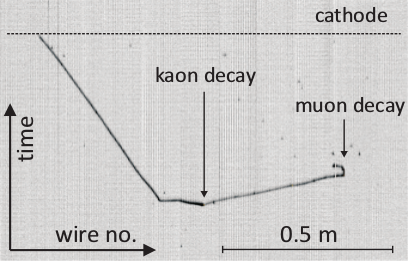
\includegraphics[width=0.8\textwidth]{fig-kaon-coll.png}
\end{dunefigure}

\begin{dunefigure}[Annotations: TikZ modified graphic]{fig:annotation-tikz}
{An image annotated using the \LaTeX Tikz package.}
\begin{tikzpicture}[scale = 1.0, font=\sffamily\LARGE]
    \node[anchor=south west,inner sep=0] at (0,0) 
    {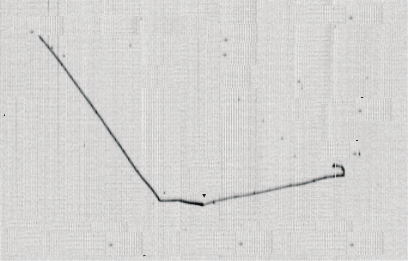
\includegraphics[width=0.8\textwidth]{fig-kaon-coll-blank.png}};
    \node at (11.7,8.5) {\textbf{cathode}};    
    \draw [line width=2pt, dotted] (0.3,7.8) -- (13.6,7.8);
    \node at (7.0,6.5) {\textbf{kaon decay}};    
    \draw [line width=1.5pt,-latex] (7.0,5.9) -- (7.0,2.1);
    \node at (11.9,5.7) {\textbf{muon decay}};    
    \draw [line width=1.5pt,-latex] (11.7,5.4) -- (11.7,3.5);
    \node at (0.9,4.1) [rotate=90] {\textbf{time}};
    \draw [line width=2pt,-latex] (0.4,0.4) -- (0.4,5.0);
    \node at (2.9,1.0) {\textbf{wire no.}};   
    \draw [line width=2pt,-latex] (0.4,0.4) -- (5.1,0.4);
    \node at (10.7,1.0) {\textbf{0.5 m}};    
    \draw [line width=1.5pt] (7.8,0.4) -- (13.5,0.4);
    \draw [line width=1.5pt] (7.8,0.2) -- (7.8,0.6);
    \draw [line width=1.5pt] (13.5,0.2) -- (13.5,0.6);    
    \draw[red,ultra thick,rounded corners] (11.3,2.5) rectangle (12.3,3.5);
\end{tikzpicture}
\end{dunefigure}


%\centerline{Figure 2.1c: \LaTeX~ TikZ Code Snippet}

\begin{dunefigure}[TikZ Code Snippet]{fig:tikz-snippet}{\LaTeX TikZ Annotation Code Snippet}
\begin{framed}
\begin{verbatim}

\begin{tikzpicture}[scale = 1.0, font=\sffamily\LARGE]
    \node[anchor=south west,inner sep=0] at (0,0) 
    {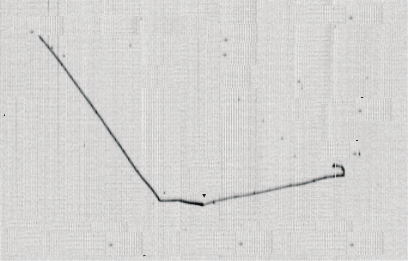
\includegraphics[width=0.8\textwidth]{fig-kaon-coll-blank.png}};
    \node at (11.7,8.5) {\textbf{cathode}};    
    \draw [line width=2pt, dotted] (0.3,7.8) -- (13.6,7.8);
    \node at (7.0,6.5) {\textbf{kaon decay}};    
    \draw [line width=1.5pt,-latex] (7.0,5.9) -- (7.0,2.1);
    \node at (11.9,5.7) {\textbf{muon decay}};    
    \draw [line width=1.5pt,-latex] (11.7,5.4) -- (11.7,3.5);
    \node at (0.9,4.1) [rotate=90] {\textbf{time}};
    \draw [line width=2pt,-latex] (0.4,0.4) -- (0.4,5.0);
    \node at (2.9,1.0) {\textbf{wire no.}};   
    \draw [line width=2pt,-latex] (0.4,0.4) -- (5.1,0.4);
    \node at (10.7,1.0) {\textbf{0.5 m}};    
    \draw [line width=1.5pt] (7.8,0.4) -- (13.5,0.4);
    \draw [line width=1.5pt] (7.8,0.2) -- (7.8,0.6);
    \draw [line width=1.5pt] (13.5,0.2) -- (13.5,0.6);    
    \draw[red,ultra thick,rounded corners] (11.3,2.5) rectangle (12.3,3.5);
\end{tikzpicture}

\end{verbatim}
\end{framed}
\end{dunefigure}

If you find the TikZ approach tedious, then at a minimum take care not to produce a 
low-quality graphic with a large filesize (>3MB). Also, please choose fonts and colors that ``work'' with the document.

If at all possible, provide the file in a format which can be further edited and which does not turn raster data into PDF nor vector data into JPEG/PNG.

If this can't be avoided and if the underlying graphic is JPEG then produce the final version in JPEG and not PNG nor PDF. If the annotation is on top of an original vector drawing and your annotation software will retain the vector information, save it as PDF.

Feel free to consult david.demuth@vcsu.edu with any assistance on creating your image annotations.
